\section{Durchführung}
\label{sec:Durchführung}

\subsection{Einseitige Einspannung}

Ein zylinder- und ein quaderförmiger Stab werden in die Apparatur eingespannt und die Nullauslenkung an verschiedenen Abständen $x$ zum Einspannpunkt mithilfe von Messuhren gemessen. Es wird am nicht eingespannten Ende ein Gewicht angehängt und erneut die Auslenkung bei verschiedenen $x$ gemessen.
\begin{figure}
	\centering
	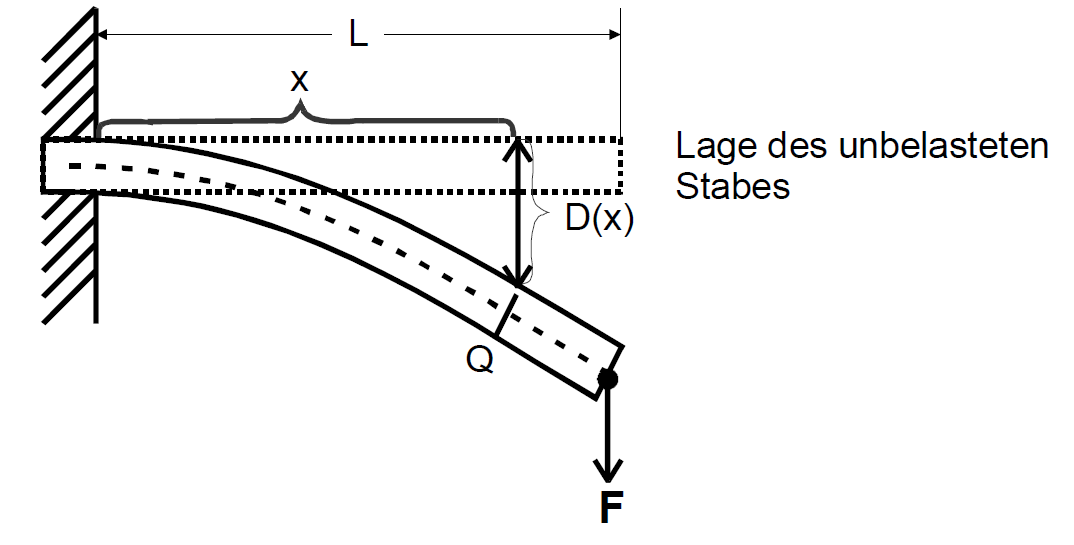
\includegraphics[scale=.295]{content/images/einseitig.png}
	\caption{Schema zur Bestimmung des Elastizitätsmoduls bei einseitiger Einspannung\cite{V103}}
	\label{fig:einseitig}
\end{figure}

\subsection{Beidseitige Auflage}

Die Enden des quaderförmigem Stabes werden auf beiden Seiten der Messapparatur aufgelegt die Nullauslenkung für verschiedene $x$ gemessen und ein Gewicht in der Mitte des Stabes.
Die resultierenden Auslenkungen werden gemessen.
\begin{figure}
	\centering
	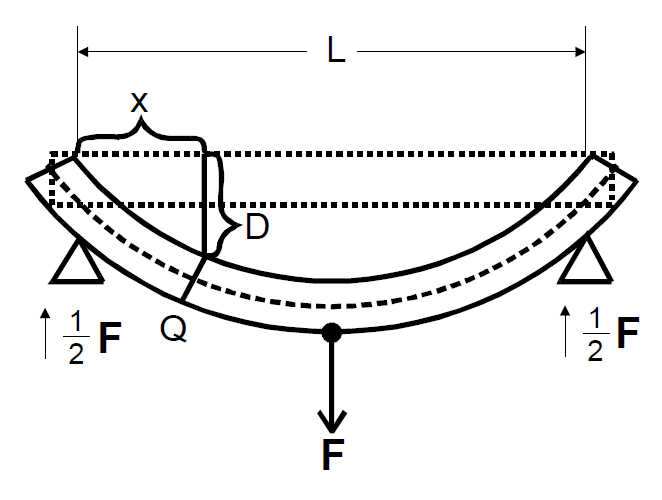
\includegraphics[scale=.305]{content/images/beidseitig.png}
	\caption{Schema zur Bestimmung des Elastizitätsmoduls bei beidseitiger Einspannung\cite{V103}}
	\label{fig:beidseitig}
\end{figure}